\chapter{Semantic Web}
\label{chap_sem_web}

\section{Introduction}

The word semantic \cite{sem1springer} itself implies meaning or understanding. As such, the fundamental difference between Semantic Web technologies and other technologies related to data (such as relational databases or the World Wide Web itself) is that the Semantic Web is concerned with the meaning and not the structure of data.\\
The semantic Web is an extension of its previous generation.  Its semantics of the resources' contents became explicit and available for the processes in a formal representation. However, these processes could infer on existing knowledge in the Web to provide more accurate and advanced information.

A brief comparison between the different versions of the Web is presented in the figure \ref{comparison} and table \ref{comparisontab} below.

\begin{figure}[H]
\centering
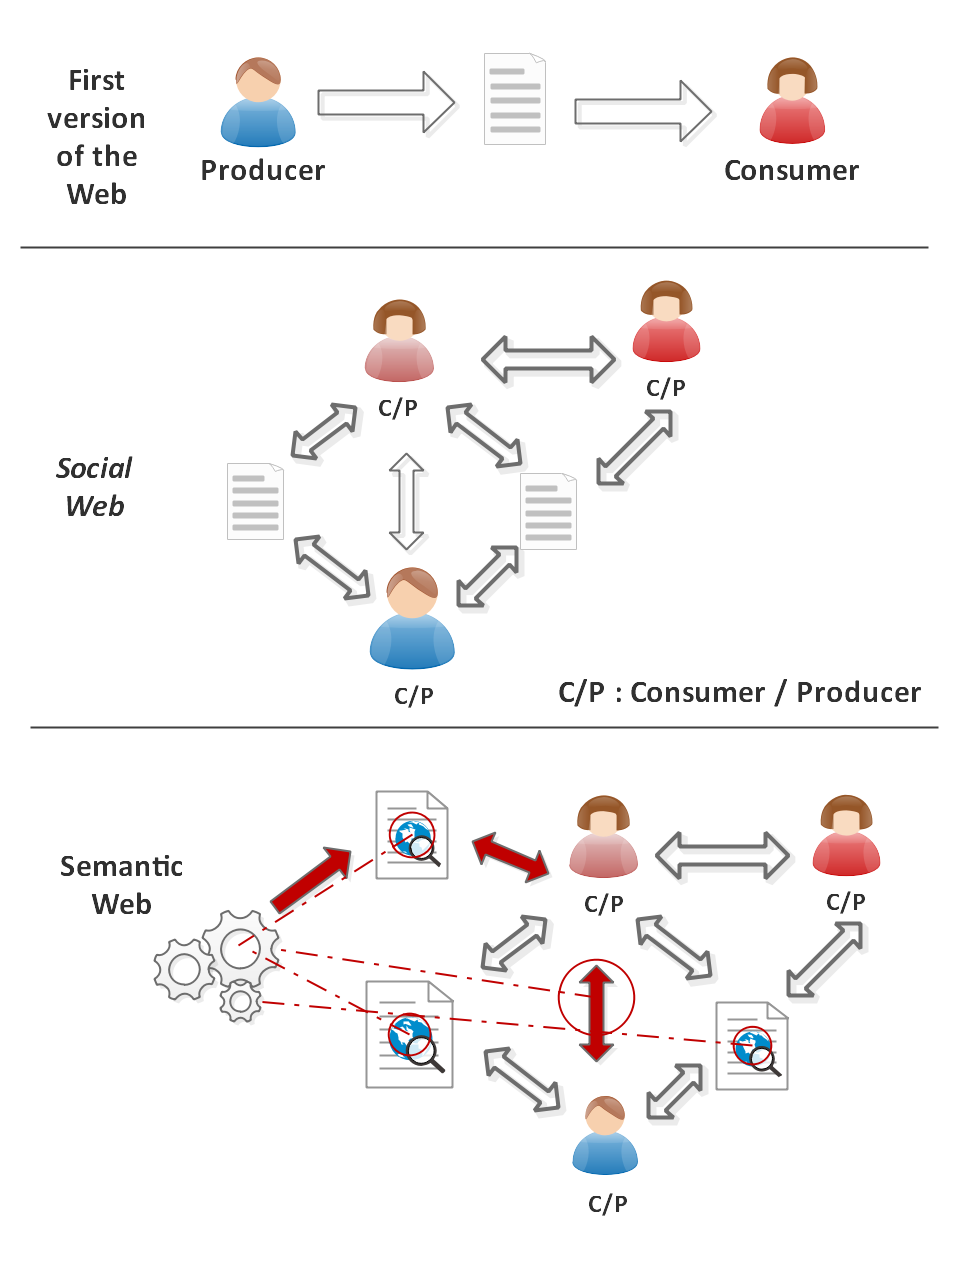
\includegraphics[scale=0.4]{peeps}
\caption{The evolution of Web}
\label{comparison}
\end{figure}



\begin{table}[H]
\centering
\caption{Web's versions comparison}
\label{comparisontab}
\begin{tabular}{|c|c|c|}
\hline
\rowcolor[HTML]{C0C0C0} 
First version of the Web        & Social Web            & Semantic Web    \\ \hline    
Dictated       & Socially constructed & Contextualy reinvented \\ \hline
Read-only      & Wildly read-write    & Portable and Personal                          \\ \hline
Company focus  & Community focus      & Individual focus                               \\ \hline
Home pages     & Blogs / Wikis        & Lifestreams / Waves                            \\ \hline

Web forms      & Web applications     & Smart applications                             \\ \hline
Owning content & Sharing content      & Consolidating content                          \\ \hline
HTML / Portals & XML/ RSS /DOM ...   & RDF /RDFS/ OWL ...                     \\ \hline
\end{tabular}
\end{table}


 
\section{Semantic Web architecture}
The architecture of semantic Web, as suggested by Tim Berners-Lee in 2000, \cite{archi} is shown in the figure \ref{fig_arch} below.  


\begin{figure}[H]
\centering
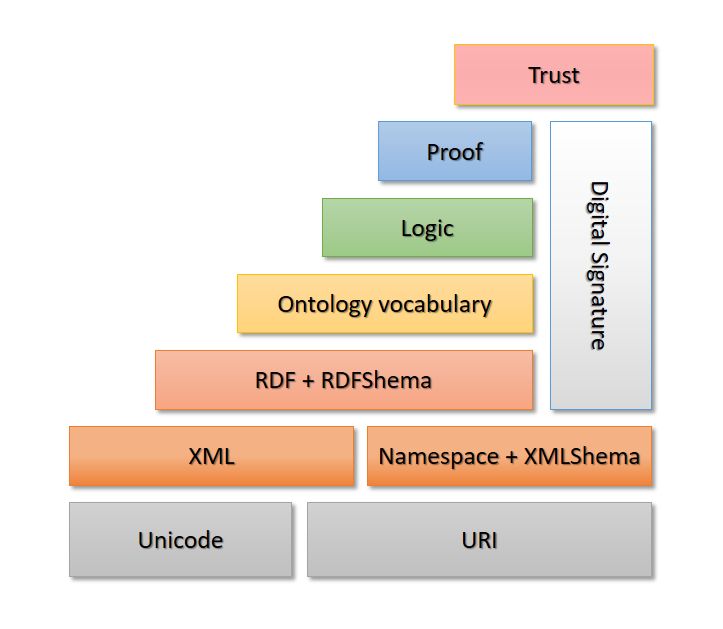
\includegraphics[scale=0.6]{arch11}
\caption{First semantic Web architecture}
\label{fig_arch}
\end{figure}


\begin{itemize}
\item The first layer is composed by URIs to give unique identifiers and Unicodes that provides every character a unique number no matter what the statform is. It allows data to be transported through many different systems without corruption.

\item In the next layer, XML allows the transportation of data between statforms, and Namespace that gives objects a referred name.

\item RDF and RDFS layers are the bases and the fundamentals of semantic Web. They describe taxonomies of concepts and properties. RDF is a simste assertions language used for describing resources in the World Wide Web. It is designed to represent information in the form of triples, such as subject, predicate and object.  

\item RDFS extends RDF vocabulary to allow describing taxonomies of classes and properties. Classes (generalized categories) and properties (predicates or binary relations) can be arranged into hierarchies. In addition, it extends definitions for some of the elements of RDF.

\item Ontologies make the collaboration between human and computers easier by sharing not only the syntax but also the semantic of Web resources.

\item The Logic layer is used to develop an advanced reasoning capabilities for knowledge extraction and efficient decision making.

\item The Proof layer defines a rule-based inference system which allows to derive assertions from known assertions described in RDF, OWL, etc.

\item Finally, the trust layer, which is based on the two previews layers (Logic and Proof), controls and determines the veracity of the information and the trust of the source of data.
\end{itemize}




%%kappa 

In 2005, W3C has suggested a new way to present the  architecture of semantic Web as we see in the figure  \ref{fig_archnew} . What is new with this architecture that is the Ontology layer is divided in two alternatives ,OWL (Ontology Web Language) a standard language to describe ontologies and Rules which is a base-rules language.

The new architecture shown in the figure \ref{fig_archnew} above is the current semantic Web standard and is subtle to change in the future.

\begin{figure}[H]
\centering
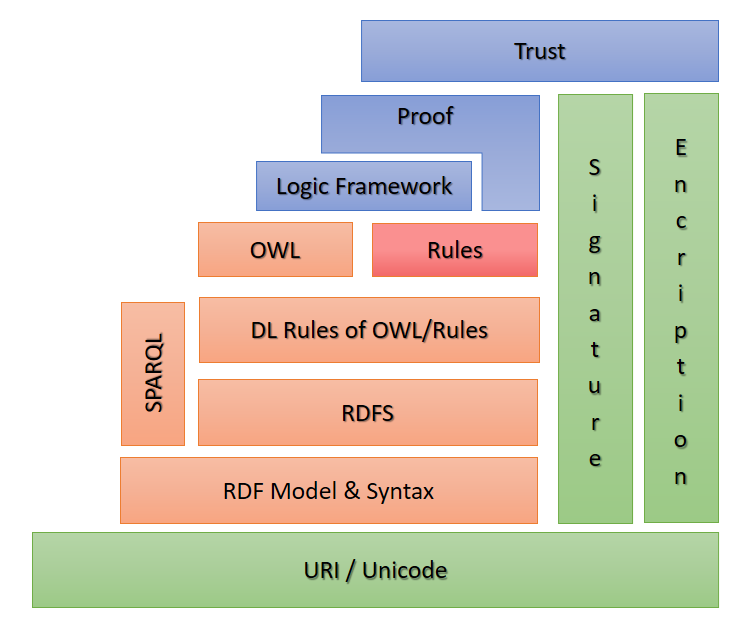
\includegraphics[scale=0.6]{arch21}
\caption{Current semantic Web architecture}
\label{fig_archnew}
\end{figure}





\section{Semantic Web Languages and technologies}
With the creation of Semantic Web, many languages were developed, most of them are based on XML or use it as a syntax. However, XML don't provide the semantic of resources, that is why other languages are used to specify the meaning of data.

\subsection{RDF}
RDF (Resource Description Framework) is a standard model for data interchange on the Web. RDF has features that facilitate data merging even if the underlying schema differ, and it specifically supports the evolution of schema over time without requiring all the data consumers to be changed.
Based on triples, RDF extends the linking structure of the Web to use URIs to name the relationship between subjects and objects. Using this simple model, it allows structured and semi-structured data to be mixed, exposed, and shared across different applications. This linking structure forms a directed, labeled graph, where the edges represent the named link between two resources, represented by the graph nodes. This graph view is the easiest possible mental model for RDF and is often used in easy-to-understand visual explanations.
Since RDF is using XML and it is at the base of the semantic Web, so that all the other languages corresponding to the upper layers are built on top of it.


RDF provides XML-based syntax, called RDF\slash XML. A piece of RDF\slash XML code written below :\\

\begin{lstlisting}[captionpos=b, caption=RDF Triple example, label={rdftriple},
basicstyle=\footnotesize,frame=single]
1. <?xml version="1.0"?>
2. <rdf:RDF xmlns:rdf="http://www.w3.org/1999/02/22-rdf-syntax-ns#"
3.          xmlns:isi="http://isi.tn#">

4.    <rdf:Description rdf:about="http://isi.tn#Student">
5.       <isi:hasName>"Safoine"</isi:hasName>
6.    </rdf:Description>

7. </rdf:RDF>       
\end{lstlisting}

\noindent Line numbers are added to the example which are explained down below:
\begin{itemize}
    \setlength{\itemsep}{0cm}
    \setlength{\parskip}{0cm}

    \item \textbf{Line 1}: contains standard XML declaration \texttt{<?xml version="1.0"?>}, which indicates that the content of that file is XML, and provides XML version which is used inside.	
    \item \textbf{Line 2}: starts from tag \texttt{rdf:RDF}, which indicates that the following XML content syntax is RDF. The \texttt{xmlns:rdf} defines a namespace identified by the URI \url{http://www.w3.org/1999/02/22-rdf-syntax-ns#}, and tells that all tags prefixed with \texttt{rdf:} are parts of the namespace. That namespace is used for terms from RDF vocabulary.
    \item \textbf{Line 3}: defines another prefix \texttt{isi:}, which represents namespace \url{http://www.isi.tn#}. URI \url{http://isi.tn#} is used for vocabulary terms defined by organization \texttt{isi.tn}.
    \item \textbf{Lines 4-6}: provide RDF/XML code, which describes the statement shown in  the graph \ref{fig_rdf}. 
    \item \textit{Line 4} begins from tag \texttt{rdf:Description} which indicates the start of description of a resource. Next, using attribute \texttt{rdf:about}, identifies the resource the statement is about (the subject of the statement), by providing its URI \url{http://isi.tn#Student}. 
    \item \textbf{Line 5}: declares property element \texttt{isi:hasName} for the subject resource, where both predicate and object of the statement are represented. The value of the property identified by namespace \url{http://isi.tn#hasName} is a stain literal \texttt{Safoine}. 
    \item \textbf{Line 6}: closes \texttt{rdf:Description} element.
    \item \textbf{Line 7}: indicates the end of \texttt{rdf:RDF} element.
\end{itemize}

\subsubsection{RDF vocabulary}
\noindent RDF vocabulary \cite{rdfv} is a defined set of predicates that can be used in an application.
The vocabulary defined by the RDF specification is indicated below:\begin{itemize}
\item \texttt{<rdf:RDF>}: Is the root element of an RDF document. It defines the XML document to be an RDF document. It also contains a reference to the RDF namespace:
\item \texttt{<rdf:Description>}: Contains elements that describe the resource.
\item \texttt{<rdf:Bag>}: Is used to describe a list of values that do not have to be in a specific order, it may contain duplicate values.
\item \texttt{<rdf:Seq>}: Is used to describe an ordered list of values.
\item \texttt{<rdf:Alt>}:is used to describe a list of alternative values (the user can select only one of the values).
\end{itemize}
Vocabulary is used as a backbone for RDF Schema, where that limited vocabulary is extended.



\subsubsection{RDF Graph}
RDF is a data model presented by a graph. The structure of every RDF model is presented by triples, each one is composed by a subject, a predicate and an object. A set of those triples forms a graph as it shown in the figure below  \ref{fig_rdf}:
\begin{itemize} 
\item Subject: The resource to describe.
\item Predicate: A property asserted to the resource.
\item Object: Is data or a other resource, it's the value of the property in the predicate.
RDF graph has at least two nodes and a property to relate them. Some of those nodes are represented by an ellipse referring to an entity with an URI ,other nodes are represented by a rectangle and having a literal value to express the entity directly.
 \end{itemize}
 \begin{figure}[H]
\centering
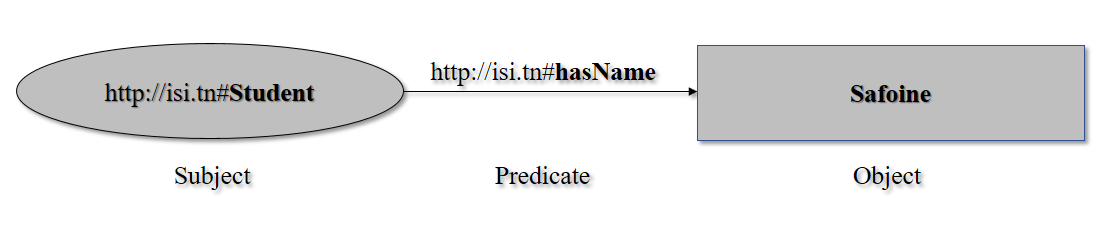
\includegraphics[scale=0.5]{rdf}
\caption{Example of RDF triple }
\label{fig_rdf}
\end{figure}


\subsubsection{Graph nodes types}
To describe Web resources, RDF graph nodes have two types: \begin{itemize}
\item URI: Is used to present resources described in RDF graph and to avoid designation confuse.
\item Literal:It describes property value and has two types: \begin{itemize}
\item Simple literal: It a string,presenting property value, it may have language attribute.
\item Typed literal: Presented by a string and an URI of that string type.
\end{itemize}
\item Empty: An empty node is an unique node that can be used in many triplets in the same RDF graph. 
\end{itemize}
RDF structure is an oriented and ordered graph based on triples. The subject of a triple may be  an URI or an empty node, the property is always presented by an URI and the object may be an URI, literal or an empty node. 

\subsubsection{RDF Graph's Relations}
An RDF triple is the description of a declaration, a logical expression or a claim in the world. RDF graph is the conjunction of triples. There are various relationships that can be established between graphs:\begin{itemize}
\item Involvement: An RDF graph A leads to an other RDF graph B, if every thing that make A true makes B also true. If A involved B, then the truth of A is proved or demonstrated then the truth of B is established.
\item Equivalence: Two RDF graphs A and B are equivalent if they describe the same information. A and B are equivalent if and only if A involved B and B involved B
\item Inconsistency: An RDF graph is inconsistent if it has an internal contradiction and there is no way that the description in the graph may be true.
\end{itemize}



\subsection{RDFS}
RDF Schema  \cite{RDFSchema} extends RDF vocabulary to allow describing taxonomies of classes and properties. Classes (generalized categories relations) and properties (predicates or binary relations) can be arranged into hierarchies. 
The RDF Schema provides a type system for RDF. The RDFS is technologically advanced compared to RDF since it provides a way to build an object model from which the actual data is referenced and which tells what things really mean. Briefly, the RDF Schema allows users to define resources with classes, properties, and values. The concept of RDF class is similar to the concept of class in object-oriented programming languages such as Java and C++. A class is a structure of similar things and inheritance is allowed (e.g: rdfs:subClassOf). This allows resources to be defined as instances of classes allowing classes to be organized in a hierarchical fashion. 
\newpage
\subsubsection{RDFS structure}
\label{sub:rdfsConstructs}

\noindent RDFS main structure and vocabulary is presented by:
\begin{itemize}
    \setlength{\itemsep}{0cm}
    \setlength{\parskip}{0cm}

\item \textbf{Classes}: Class tag are described in the table \ref{class_tag} below:
\begin{table}[H]
\centering
\caption{RDFS Class tags}
\label{class_tag}
\begin{tabular}{|l|l|}
\hline
rdfs:Resource  & All things described by RDF are resources, it is the class of everything \\ \hline
rdfs:Class     & Declares a resource as a class of another resource                       \\ \hline
rdfs:Literal   & Literal values, such as strings or integers                              \\ \hline
rdfs:Datatype  & It's a class of datatypes                                                \\ \hline
rdf:XMLLiteral & The class of XML literal values                                          \\ \hline
rdf:Property   & Class of properties                                                      \\ \hline
\end{tabular}
\end{table}

   %% \item \textbf{Classes}: \texttt{rdfs:Resource}: All things described by RDF are resources, it is the class of everything. \texttt{rdfs:Class}: Declares a resource as a class of another resource. \texttt{rdfs:Literal}: Literal values, such as strings or integers. \texttt{rdfs:Datatype}: It's a class of datatypes. \texttt{rdf:XMLLiteral}: The class of XML literal values. and \texttt{rdf:Property}: Class of properties. Example:
%%\textbf{Example}:
%%{\tt \small
%%\begin{verbatim}
%%<rdf:Description rdf:about="http://isi.tn#Student">
 %%  <rdf:type rdf:resource=Mehdi/>
%%</rdf:Description>
%%\end{verbatim}
%%}
%%
%%{\tt \small
%%\begin{verbatim}
%%<rdfs:Class rdf:ID="StudentID">
 %%  <rdfs:subClassOf rdf:resource="L3FSI01"/>
%%</rdf:Class>
%%\end{verbatim}
%%}

    \item \textbf{Properties}: Property tags are shown in table \ref{prop_tag} below:
    
\begin{table}[H]
\centering
\caption{RDFS Property's tags}
\label{prop_tag}
\begin{tabular}{|l|l|}
\hline
rdfs:domain        & Declares the class of the \texttt\{subject\} in a triple block   \\ \hline
rdfs:range         & Declares the class or datatype of the object in a triple block   \\ \hline
rdf:type           & Property used to state that a resource is an instance of a class \\ \hline
rdfs:subClassOf    & Allows to declare hierarchies of classes                         \\ \hline
rdfs:subPropertyOf & Allows to declare hierarchies of properties                      \\ \hline
rdfs:seeAlso       & Relates a resource to another with additional exstanation        \\ \hline
rdfs:isDefinedBy   & Relates a resource to its definition                             \\ \hline
rdfs:label         & Provides friendly name of resource                               \\ \hline
rdfs:comment       & Provides a human-readable description of a resource              \\ \hline
\end{tabular}
\end{table}
    
    %%\texttt{rdfs:domain}: Declares the class of the \texttt{subject} in a triple block. \texttt{rdfs:range}: Declares the class or datatype of the object in a triple block. \texttt{rdf:type}: Property used to state that a resource is an instance of a class. \texttt{rdfs:subClassOf}: Allows to declare hierarchies of classes. \texttt{rdfs:subPropertyOf} Allows to declare hierarchies of properties.\texttt{rdfs:seeAlso}: Relates a resource to another with additional exstanation.
     %% \texttt{rdfs:isDefinedBy}: Relates a resource to its definition.
     %%\texttt{rdfs:label}: Provides friendly name of resource.
      %%\texttt{rdfs:comment}: Provides a human-readable description of a resource).\\
     

%%{\tt \small
%%\begin{verbatim}
%%<rdf:Property rdf:ID="StudentID">
  %% <rdfs:subPropertyOf rdf:resource="isStudent"/>
   %%<rdfs:domain rdf:resource="Peoste"/>
   %%<rdfs:ranage rdf:resource="isiStudents"/>
%%</rdf:Property>
%%\end{verbatim}
%%}

      
\end{itemize}

%%\medskip

\noindent The fact is, that there is lack of any notion of negation or disjunction in RDFS. It provides only a very limited notion of existential quantification. This makes for RDFS language \textit{"very limited expressive power"}.

\subsection{Ontology}
The term ontology \cite{ontonew} derives from Greek, with “onto” meaning “being”, and “logos” usually interpreted as “science”; so that ontology, as traditionally understood, is the science or study of being.
Ontologies in computer science are conceptual schema that provides a logical description of data. An ontology defines terms which with to represent knowledge. For present purposes, one can think of data as that expressible in ground atomic facts and knowledge as that expressible in logical sentences with existentially and universally quantified variables. An ontology defines the vocabulary used to compose complex expressions such as those used to describe resource constraints in a stunning  problem. From a finite, well-defined vocabulary one can compose a large number of coherent sentences. That is one reason why vocabulary, rather than form, is the focus of specifications of ontological commitments. 

Ontologies are classified according to its subject and its structure, we recognize:\begin{itemize}  
\item \textbf{Domain ontologies}: This type of ontology is the most used in semantic Web applications, it describes resources of a specific domain and can be reuse in different applications in the same domain.

\item\textbf{Application ontologies}: It contains knowledge which are necessarily for a given application.
\item \textbf{Generic ontologies}: A high level ontology because it describes very generic resources like time, space, state, process,etc.
The concepts contained in an ontology of the domain are included in the concepts of a generic ontology.
\end{itemize} 
The conception of an ontology consider the fact that the semantic Web is distributed, that's why we can extend existing ontologies, or use them to create new ones .
To use terms in the ontology, we must indicate from what ontology it comes, that why we use prefixes that every ontology should  begin with in \textit{rdf:RDF} tag.
After that comes the content of the ontology putted in \textit{Owl:Ontology} tag.
The different component of an ontology are classes,properties and individuals.

\textbf{Classes}: A class in a group of individuals that have similar characteristics and may be classed hierarchically by a taxonomy.
All defined classes are children of a super-class called. \textit{OWL:Thing}. As the oriented object languages, inheritance is available in ontologies using the property \textit{subClassOf} of rdfs.

\textbf{Properties}: A property expresses a fact about a class and their individuals e.g the color of a car, it model and power are properties of car class.
There are two types of properties:\begin{itemize}
\item Properties allow to link individuals to other individuals.
\item Properties of data type allow to give a literal value to an individual.
\end{itemize}

\textbf{Individuals}: The definition of an individual is expressing a fact about a class, individuals are also called axioms and there are two types of them:\begin{itemize}
\item Fact that belongs to a class, indeed we declare an individual and its property's literal value.
\item Fact concerning individual's identity, we may face problems when axioms in a class are not unique and to solve that ambiguity we use properties like \textit{owl:sameAs},\\             \textit{owl:differentFrom} and \textit{owl:allDifferent}.
\end{itemize}

\subsection{OWL}
OWL (Ontology Web Language) \cite{OWL} is a W3C recommendation since 2004 . On top of RDF and RDFS, OWL comes with a larger vocabulary and stronger syntax, having a similar foundation as other Semantic Web languages, OWL has greater machine interpret ability. OWL provides a variety of constructors to express properties(roles), objects(individuals) and classes(concepts) as showed below:  \begin{itemize}
    \item Connectors of logical description (intersection, union, various restrictions..)
    \item Properties of defined classes
    \item Cardinality
    \item Types of properties
    \item Characteristics of properties (e.g. symmetry, transitivity)
\end{itemize}

The table \ref{tab:owlConstructors} \cite{HLP08} below presents different OWL constructors and their DL Syntax equivalent. 

\begin{table}[H]
\centering
\begin{tabular}{ |>{\tt}l|l|l| }
    \hline
    \multicolumn{1}{|c|}{\textbf{Constructor}}  & \multicolumn{1}{c|}{\textbf{DL Syntax}}   & \multicolumn{1}{c|}{\textbf{Example}} \\ \hline
    intersectionOf                              & $C_{1}\sqcap\cdots\sqcap C_{n}$           & $Human \sqcap Male$ \\ \hline
    unionOf                                     & $C_{1}\sqcup\cdots\sqcup C_{n}$           & $\mathit{Doctor} \sqcup \mathit{Lawyer}$ \\ \hline
    comstementOf                                & $\lnot C$                                 & $\lnot \mathit{Male}$ \\ \hline
    oneOf                                       & ${x_{1}\cdots x_{2}}$                     & ${\mathit{john},\mathit{mary}}$ \\ \hline
    allValuesFrom                               & $\forall P.C$                             & $\forall \mathit{hasChild}.\mathit{Doctor}$ \\ \hline
    someValuesFrom                              & $\exists r.C$                             & $\exists \mathit{hasChild}.\mathit{Lawyer}$ \\ \hline
    hasValue                                    & $\exists r.\{x\}$                         & $\exists \mathit{citizensOf}.\{\mathit{USA}\}$ \\ \hline
    minCardinality                              & $(\geq nr)$                               & $(\geq 2~\mathit{hasChild})$ \\ \hline
    maxCardinality                              & $(\leq nr)$                               & $(\leq 2~\mathit{hasChild})$ \\ \hline
    inverseOf                                   & $r^{-}$                                   & $\mathit{hasChild}^{-}$ \\ \hline
\end{tabular}
\caption{OWL constructors}
\label{tab:owlConstructors}
\end{table}

OWL is based on axioms, those axioms are used to make assertions,e.g assertions of relationships between classes or properties.
%%TABLEAU 

Furthermore, the table \ref{tab:owlAxioms} \cite{HLP08} below presents different axioms on the OWL syntax and their DL Syntax equivalent. 

\begin{table}[H]
\centering
\begin{tabular}{ |>{\tt}l|l|l| }
    \hline
    \multicolumn{1}{|c|}{\textbf{Axiom}}    & \multicolumn{1}{c|}{\textbf{DL Syntax}}   & \multicolumn{1}{c|}{\textbf{Example}} \\ \hline
    subClassOf                              & $C_{1} \sqsubseteq C_{2}$                 & $\mathit{Human} \sqsubseteq \mathit{Animal} \sqcap \mathit{Biped}$ \\ \hline
    equivalentClass                         & $C_{1} \equiv C_{2}$                      & $\mathit{Man} \equiv \mathit{Human} \sqcap \mathit{Male}$ \\ \hline
    subPropertyOf                           & $P_{1} \sqsubseteq P_{2}$                 & $\mathit{hasDaughter} \sqsubseteq \mathit{hasChild}$ \\ \hline
    equivalentProperty                      & $P_{1} \equiv P_{2}$                      & $\mathit{cost} \equiv \mathit{price}$ \\ \hline
    disjointWith                            & $C_{1} \sqsubseteq \lnot C_{2}$           & $\mathit{Male} \sqsubseteq \lnot \mathit{Female}$ \\ \hline
    sameAs                                  & ${x_{1}} \equiv {x_{2}}$                  & $\mathit{President\_Bush} \equiv \mathit{G\_W\_Bush}$ \\ \hline
    differentFrom                           & ${x_{1}} \sqsubseteq \lnot {x_{2}}$       & $\mathit{john} \sqsubseteq \lnot \mathit{peter}$ \\ \hline
\end{tabular}

\caption{OWL axioms}
\label{tab:owlAxioms}
\end{table}


Using DL syntax ,we are able create OWL equivalents by serializing them into XML as shown below :
\[
\mathit{Female} \sqcap \mathit{Male}
\]

{\tt \small
\begin{verbatim}
<owl:intersectionOf rdf:parseType="Collection">
   <rdf:Description rdf:about="#Female"/>
   <rdf:Description rdf:about="#Male"/>
</owl:intersectionOf>
\end{verbatim}
}

\[
\mathit{Student} \sqcup \mathit{Professor}
\]

{\tt \small
\begin{verbatim}
<owl:unionOf rdf:parseType="Collection">
   <rdf:Description rdf:about="#Student"/>
   <rdf:Description rdf:about="#Professor"/>
</owl:unionOf>
\end{verbatim}
}

\[
\exists \mathit{hasChild}.\mathit{Lawyer}
\]

{\tt \small
\begin{verbatim}
<owl:Restriction>
   <owl:onProperty rdf:resource="#hasChild"/>
   <owl:someValuesFrom rdf:resource="#Lawyer"/>
</owl:Restriction>
\end{verbatim}
}

\[
\exists \mathit{citizensOf}.\{\mathit{Tunisia}\}
\]

{\tt \small
\begin{verbatim}
<owl:Restriction>
   <owl:onProperty rdf:resource="#isCitizenOf"/>
   <owl:hasValue rdf:resource="#Tunisia"/>
</owl:Restriction>
\end{verbatim}
}

\bigskip

\subsubsection{OWL and reasoners}
One of reasons why OWL is based on DL is that we can use DL reasoning services in OWL based applications. The decidable ensures, that consistency of OWL DL ontology can be checked by DL reasoners. Reasoners can be also used to infer information from asserted facts.\\
The most popular reasoners in OWL community are :Pellet, FaCT, FaCT++, KAON2 or HermiT, RACER.
These reasoners provide reasoning services for tools that create and maintain ontologies like Protégé, Swoop, OilEd and TopBraid Composer.\\
The number of tools designed for OWL have increased , that motivate the community to develop ontologies for various fields like medicine, geology, biology, geography, astronomy, agriculture or defence, in which ontologies are adopted.

\subsubsection{OWL sublanguages}
There are three variants of OWL that W3C specification defines. These sublanguages are:OWL Lite, OWL DL and OWL Full that provides different level of expressiveness (increasingly in mentioned order) \cite{semwebp}. Each one of them is an extension of its predecessor. 
We have three sublanguages in OWL: \begin{itemize}
\item  \textbf{OWL Lite}: The simplest version, it support the classification hierarchies with simple constraints. It's not widely used  and acts as the entry point for Semantic Web application developers.
\item  \textbf{OWL DL}: Includes OWL Lite, it's the most used version of OWL. It was designed to provide maximum expressiveness possible while retaining computational decidable and automated reasoning.
\item  \textbf{OWL Full}: The most powerful OWL version in expressiveness. Includes OWL DL. Provides different semantic than predecessors.
\end{itemize}
\subsubsection{OWL 2}
OWL2 \cite{OWL2} has the same structure of OWL1 almost all of it components are present. OWL adds more functionality with respect to OWL1. Some of the new features are syntactic sugar while others offer new expressively, including:\begin{itemize}
\item Keys
\item Property chains
\item Richer data types, data ranges
\item Qualified carnality restrictions
\item Asymmetric, reflexive, and disjoint properties
\item Enhanced annotation capabilities 
\end{itemize}

OWL2 can be represented in a new format that is called the Manchester Syntax, its main objective is to ease the read/write process of DL Ontologies.\\
Also OWL2 has also its own sub-languages (profiles), we can mention:
\begin{itemize}
\item \textbf{OWL2 EL}: It is particularly suitable for applications where very large ontologies are needed. It enables polynomial time algorithms for all the standard reasoning tasks.
\item  \textbf{OWL2 QL}: Enables conjunctive queries to be answered in LogSpace using standard relational database technology; it is particularly suitable for applications where relatively lightweight ontologies are used to organize large numbers of individuals and where it is useful or necessary to access the data directly via relational queries(e.g. SQL).
\end{itemize}
\subsection{SPARQL}
SPARQL(SPARQL Protocol And RDF Query Language) \cite{SPARQL} is a W3C recommendation since January 2008 as a standard to query data in RDF graphs. A SPARQL query is a definition of a graph pattern through variables and constants. 

SPARQL has several query forms. These query forms use the solutions from pattern matching to form result sets or RDF graphs. 
For example, we will perform different SPARQL queries on the triple shown on the listing \ref{sparqltriple} below:

\begin{lstlisting}[captionpos=b, caption=Queried RDF triple, label={sparqltriple},
basicstyle=\footnotesize,frame=single]
// <http://exemple.isi/book/book1> <http://purl.org/dc/terms/title> "Learning C++"   
\end{lstlisting}

\begin{itemize}

\item \textbf{SELECT}: The query consists of two parts: the SELECT clause identifies the variables to appear in the query results, and the WHERE clause provides the basic graph pattern to match against the data graph.\\



QUERY:
{\tt \small
\begin{verbatim}
SELECT ?title
WHERE{
<http://example.isi.tn/book/book1> <http://purl.org/dc/terms/title> ?title.
}  
\end{verbatim}
}

RESULT: 
\bigskip
\begin{table}[H]
\centering
\caption{SPARQL query result}
\label{my-label}
\begin{tabular}{|c|}
\hline
?title         \\ \hline
"Learning C++" \\ \hline
\end{tabular}
\end{table}

\item \textbf{ASK}: Return true if the query match data in RDF, otherwise return false.\\
{\tt \small
\begin{verbatim}
@prefix foaf:       <http://xmlns.com/foaf/0.1/> .
:a  foaf:name       "Mehdi" .
:a  foaf:homepage   <http://work.example.isi.tn/Mehdi/> .
:b  foaf:name       "Safoine" .
:b  foaf:mbox       <mailto:safoine@example.isi.tn> .
\end{verbatim}
}
\newpage
QUERY: 
{\tt \small
\begin{verbatim}
PREFIX foaf:    <http://xmlns.com/foaf/0.1/>
ASK  { ?person foaf:name  "Mehdi". }
\end{verbatim}
}
RESULT: True.
\item \textbf{CONSTRUCT}: Returns an RDF graph by restricting the values in the data models.\\
QUERY:
{\tt \small
\begin{verbatim}
PREFIX foaf:    <http://xmlns.com/foaf/0.1/>
PREFIX vcard:   <http://www.w3.org/2001/vcard-rdf/3.0#>
CONSTRUCT   { <http://example.isi.tn/person#Mehdi> vcard:FN ?name }
WHERE   { ?x foaf:name ?name .}
\end{verbatim}
}
RESULT: 
{\tt \small
\begin{verbatim}
@prefix vcard: <http://www.w3.org/2001/vcard-rdf/3.0#>\\
<http://example.isi.tn/person#Mehdi> vcard:FN "Mehdi" .\\
\end{verbatim}
}
\item \textbf{DESCRIBE}: Returns a RDF graph who sets the corresponding resource.\\
\textbf QUERY:
{\tt \small
\begin{verbatim}
PREFIX foaf:   <http://xmlns.com/foaf/0.1/>
DESCRIBE ?x
WHERE    { ?x foaf:name "Mehdi". }
\end{verbatim}
}
\textbf{RESULT}:
{\tt \small
\begin{verbatim}
@prefix foaf:       <http://xmlns.com/foaf/0.1/> .
:a  foaf:name       "Mehdi" .
:a  foaf:homepage   <http://work.example.isi.tn/Mehdi/> .
\end{verbatim}
}
\end{itemize} 
\subsection{Annotation}
Semantic annotation is the process of attaching additional information to various concepts (e.g. people, things, places, organizations etc) in a given text or any other content. Unlike classic text annotations for reader’s reference, semantic annotations are used by machines to refer to.
When a document (or another piece of content, e.g. video) is semantically annotated it becomes a source of information that is easy to interpret, combine and reuse by our computers. Annotation can be manual, semi-automatic (based on automatic suggestions), or fully automatic. Manual annotation tools allow users to add annotations to web pages or other resources, and share these with others. An example annotation would relate the text “Paris” to ontology, identifying it as a city and as capital of "France". Automatic tools can perform similar annotations (such as named-entity recognition \cite{nlp}) without manual intervention. 

\section*{Conclusion}
The Semantic Web is not a dependant technology but an
extension of the old ones, in which the information is given a well-defined meaning, a better enabling computers and people to work in cooperation. The first steps in weaving the semantic Web into the structure of the existing Web are already and still under way. In the near future, these developments will usher in significant new functionality as machines become more intelligent and able to process and "understand" the data that they merely display at present. The Semantic Web will bring structure to the meaningful content of Web pages, creating an environment where software agents roaming from page to page can readily carry out sophisticated tasks for users. 
